\documentclass{beamer}
    %
    % Choose how your presentation looks.
    %
    % For more themes, color themes and font themes, see:
    % http://deic.uab.es/~iblanes/beamer_gallery/index_by_theme.html
    %
    \mode<presentation>
    {
      \usetheme{default}      % or try Darmstadt, Madrid, Warsaw, ...
      \usecolortheme{default} % or try albatross, beaver, crane, ...
      \usefonttheme{default}  % or try serif, structurebold, ...
      \setbeamertemplate{navigation symbols}{}
      \setbeamertemplate{caption}[numbered]
    }

    \usepackage[english]{babel}
    \usepackage[utf8x]{inputenc}
    \usepackage{graphicx}
    \graphicspath{ {imgs/} }

    \title[Toward Controlled Generation of Text]{Toward Controlled Generation of Text}
    \author{Agustinus Kristiadi and Yonathan Santosa}
    \institute{University of Bonn}
    \date{21 Dec 2017}

    \begin{document}

    \begin{frame}
      \titlepage
    \end{frame}

    % Uncomment these lines for an automatically generated outline.
    \begin{frame}{Outline}
     \tableofcontents
    \end{frame}


    \section{Introduction}

    \subsection{Quick Introduction to Generative Models}

    \begin{frame}{Generative Model}

    \begin{itemize}
        \item Recall Bayes' Rule:
        $$P(\theta \vert X) = \frac{P(X \vert \theta) P(\theta)}{P(X)}$$
        \item Generative Model: modeling $P(X)$.
        \item Important models: GAN, VAE.
        \item In our work we will be based on VAE.
    \end{itemize}

    \end{frame}

    \subsection{Autoencoder}

    \begin{frame}{Autoencoder (AE)}

      \begin{itemize}
          \item Neural nets that take input $X$ and to reconstruct it, i.e. outputting $\hat{X}$

      \end{itemize}

      \begin{figure}
        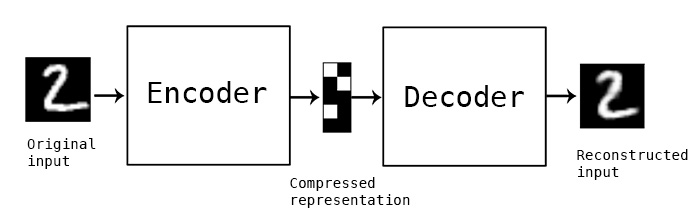
\includegraphics[width=\textwidth]{ae}
        \caption{\label{fig:ae}From: https://blog.keras.io}
        \end{figure}

    \end{frame}

    \subsection{Variational Autoencoder}

    \begin{frame}{Variational Autoencoder (VAE) \footnote{Kingma and Welling, 2013}}

        \begin{itemize}
            \item Constraint the hidden layer into some distribution (of latent variable).
            \item Force the hidden layer to match our prior distribution, e.g. standard normal.
            \item Objective: maximize (reconstruction + hidden unit regularization)

            $$\max_{\theta} \mathcal{L}(\theta;X) = \mathbb{E}_{q(z \vert X)}[\log p(X \vert z)] - D_{KL}[q(z \vert X) \Vert p(z)]$$

            \item In practice: $q(z \vert X)$ and $p(X \vert z)$, are neural nets.
        \end{itemize}

    \end{frame}

    \begin{frame}{Benefits of VAE}
        \begin{itemize}
            \item Latent variables nicely contained in $\mathcal{N}(0, I)$.
            \item Generating data $X$ becomes possible: $z \sim \mathcal{N}(0, I); X \sim P(X \vert z)$.
        \end{itemize}

        \begin{figure}
            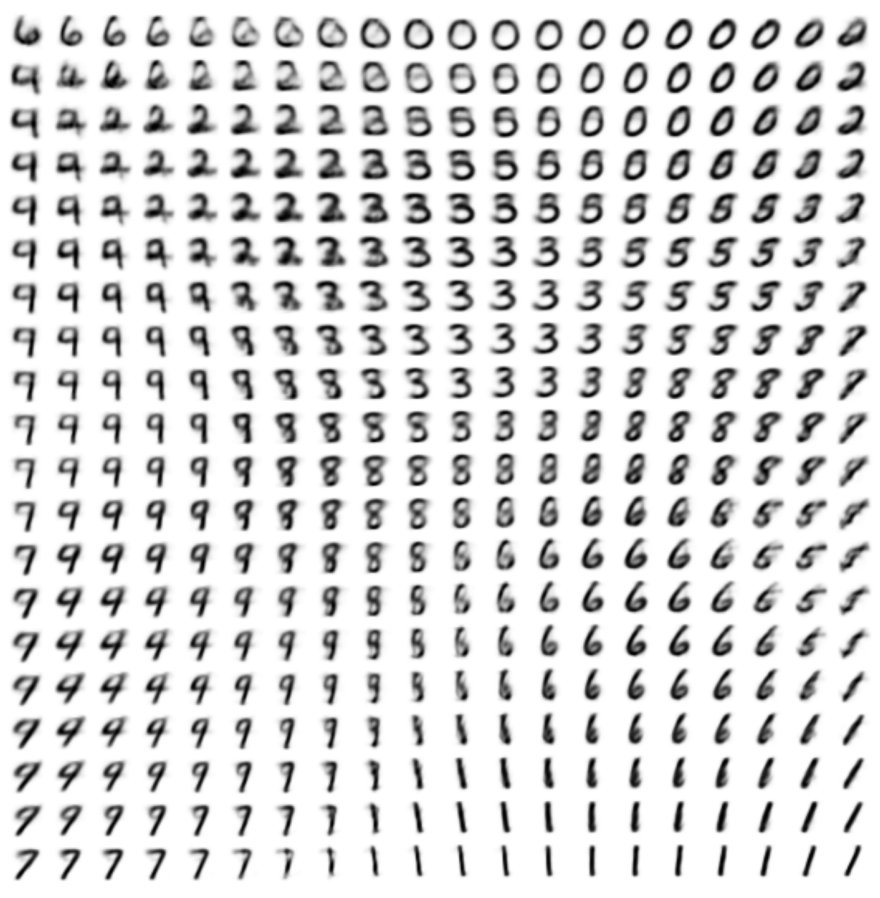
\includegraphics[width=0.5\textwidth]{vaeinterpolation}
            \caption{\label{fig:interpolation} By interpolating $z$ and transform it with $P(X \vert z)$ we can interpolate data. From: https://ermongroup.github.io/cs228-notes.}
        \end{figure}
    \end{frame}

    \section{Controlled Generation of Text}

    \subsection{Introduction}

    \begin{frame}{Toward Controlled Generation of Text (Hu, 2017)}

        \begin{itemize}
            \item Extending VAE model
            \begin{itemize}
                \item Use LSTM-RNNs as encoder and decoder.
                \item Add another neural net to enforce conditional attribute constraint.
            \end{itemize}
            \item Enables us to condition text generation. \\E.g. generate text with past tense and positive sentiment: \\"this was spectacular , i saw it in theaters twice".
        \end{itemize}

    \end{frame}

    \subsection{Algorithm}

    \begin{frame}{Architecture}
        \begin{figure}
            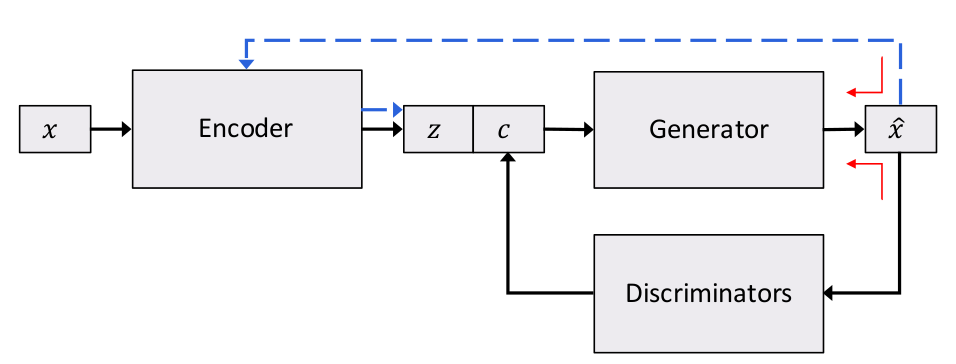
\includegraphics[width=0.8\textwidth]{architecture}
            \caption{\label{fig:arch}Hu, et al., 2017}
        \end{figure}

        \begin{itemize}
            \item We are optimizing:
            $$\min_{\theta_G, \theta_E} \mathcal{L}_{VAE} + \lambda \mathcal{L}_{attr}$$
            $$\min_{\theta_{D}} \mathcal{L}_D = \mathcal{L}_s + \lambda_u \mathcal{L}_u $$
            where $\mathcal{L}_{attr}$ is loss function for conditional attribute constraint.
        \end{itemize}
    \end{frame}

    \begin{frame}{Algorithm}
        \begin{figure}
            \includegraphics[width=\textwidth]{Algorithm}
            \caption{\label{fig:algo}Hu, et al., 2017}
        \end{figure}
    \end{frame}

    \subsection{Expected Results}

    \begin{frame}{Example Expected Results}
        \begin{figure}
            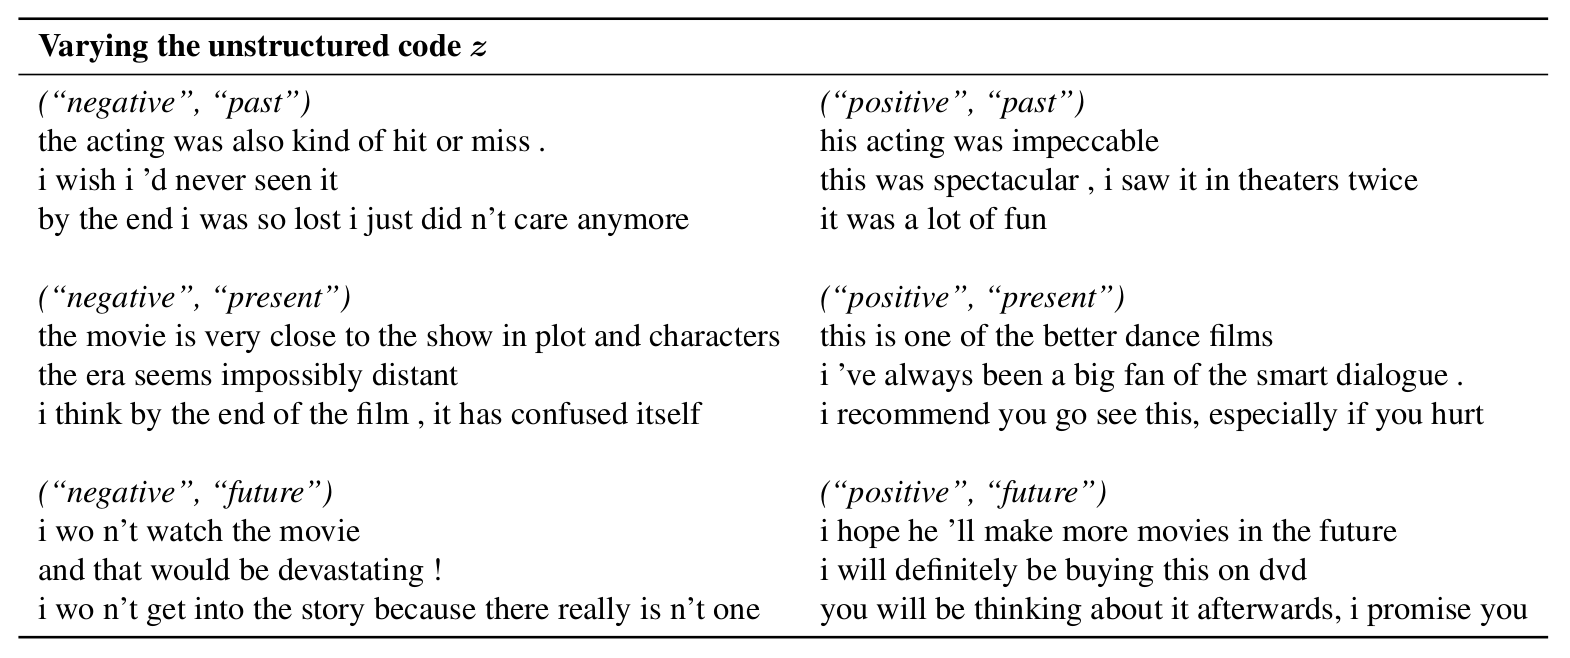
\includegraphics[width=\textwidth]{example}
            \caption{\label{fig:example}Hu, et al., 2017}
        \end{figure}
    \end{frame}

    \section{Conclusion}

    \begin{frame}{Conclusion}
        \begin{itemize}
            \item VAE is a useful modification of original autoencoder.
            \item We can extend VAE to also learn conditional constraint.
            \item We can generate text with desired properties based on the conditional constraint.
        \end{itemize}
    \end{frame}

    \begin{frame}{References}

        \begin{itemize}
            \item Kingma, Diederik P., and Max Welling. "Auto-encoding variational bayes." arXiv preprint arXiv:1312.6114 (2013). \href{https://arxiv.org/abs/1312.6114}{[pdf]}
            \item Hu, Zhiting, et al. "Toward controlled generation of text.” ICML 2017. \href{http://proceedings.mlr.press/v70/hu17e/hu17e.pdf}{[pdf]}
        \end{itemize}
    \end{frame}

\end{document}
